\documentclass[]{article}

\usepackage{graphicx}

\begin{document}

\title{Dealing With Direction-Dependent Effects In WSRT Data: Luxury Problems, Or Signposts To SKA calibration?}

\author{O. Smirnov}

\maketitle

The WSRT has turned 40 this year, but despite the respectable age, it still retains the world dynamic range crown. The image of Figure 1 is an example. It shows the field around the bright source 3C147 at 21cm. The image was has a DR of 1,600,000:1, when no other instrument has yet exceeded a million! This DR was achieved by Ger de Bruyn using the NEWSTAR package, with only a single 12-hour synthesis.

\begin{figure}
\includegraphics[width=\textwidth]{fig1-3C147-rgb}
\caption{A 21cm WSRT map of 3C147, at a dynamic range of 1,600,000:1, and absolutely no off-axis artifacts.}
\end{figure}
 
The image is even more remarkable for what it {\em doesn't} show. Traditional selfcal, such as that done by NEWSTAR, does not deal with direction-dependent effects (DDEs; also called {\em off-axis errors}), which manifest themselves as artifacts around off-center sources (left inset). Due to its careful design, WSRT has a comparatively low level of DDEs, so they only become apparent when we reach such high dynamic ranges -- some may even call it a ``luxury problem.'' To eliminate DDEs (right inset), we have reduced Ger's data again using MeqTrees, applying {\em differential gain solutions} ($\Delta E$) in the direction of the off-center sources. The result is the completely artifact-free, noise-limited image of Fig. 1.

\begin{figure}
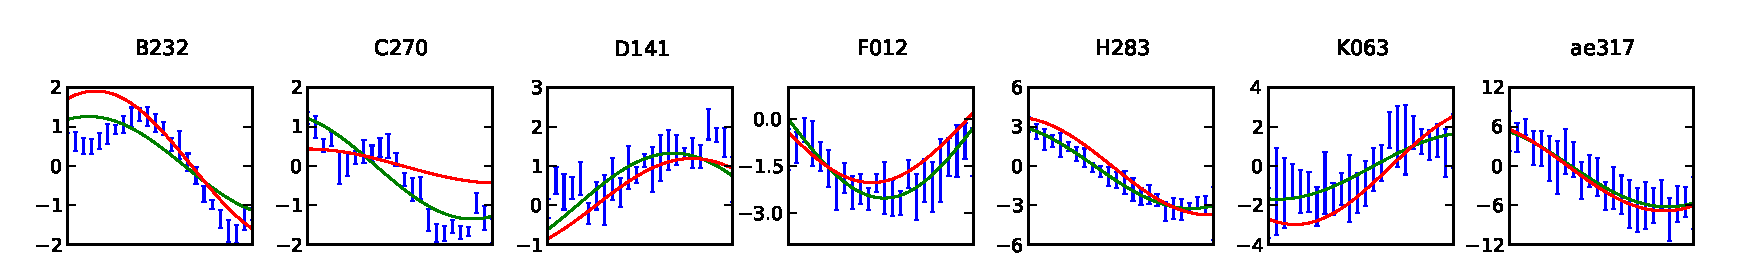
\includegraphics[width=\textwidth]{o2003_dEphase_array_slopes}
\caption{Measured phase slopes (in deg/km) of the $\Delta E$ solutions towards six off-axis sources in the 3C147 field. Green curves indicate the best-fitting positional offsets. Red curves correspond to a global rotation of $45''$. }
\end{figure}

The $\Delta E$ solutions had their own story to tell. They seemed to show  time-variable phase slopes over the array, which in turn proved to be consistent with a rotational offset of the whole field (Fig. 2). This must be due to some subtle systematic error which we have yet to chase down. In the meantime, we realized that this tecnnique could be used to probe DDEs using quite faint (as faint as 2 mJy!) sources. We therefore looked for a suitable field full of off-center sources to explore this approach further, for example to see if pointing errors could be detected. Two such fields were identified: QMC and QMC2 (named in honour of the long-defunct WSRT Quality Monitoring Committee.) We were allocated two observations of the QMC2 field, a ``Reference'' run with perfect pointing, and a ``Challenge'' run with deliberate (and secret) pointing errors on a few antennas, which were only known to Hans van Someren. The challenge was to see whether these could be recovered from the data.

Much to our surprise, the Reference observation didn't look all that perfect! The $\Delta E$  solutions ``pointed'' to a gross mispointing on antenna RT8. We notified radio observatory staff of this ``prediction from the data'', and they promptly discovered a mechanical fault on the telescope. 

\newlength{\roguewidth}
\setlength{\roguewidth}{.2\textwidth} 
\begin{figure}
\begin{tabular}{@{}c@{}c@{}c@{}c@{}c@{}}
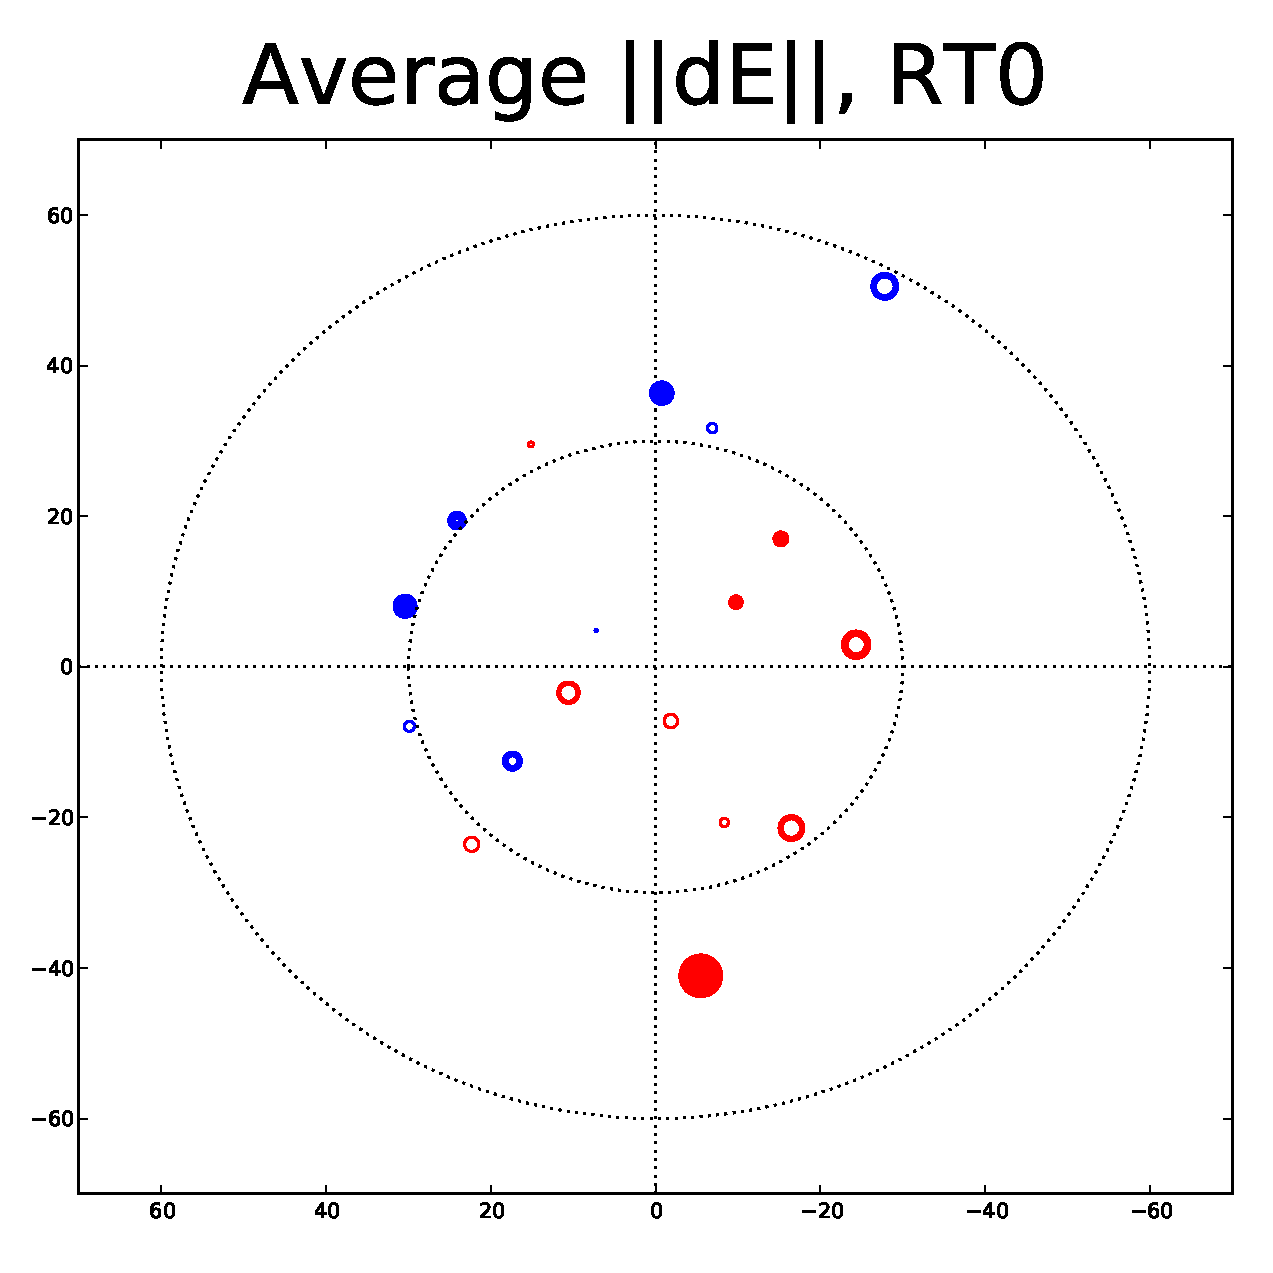
\includegraphics[width=\roguewidth]{qmc2b_dE_ant0} &
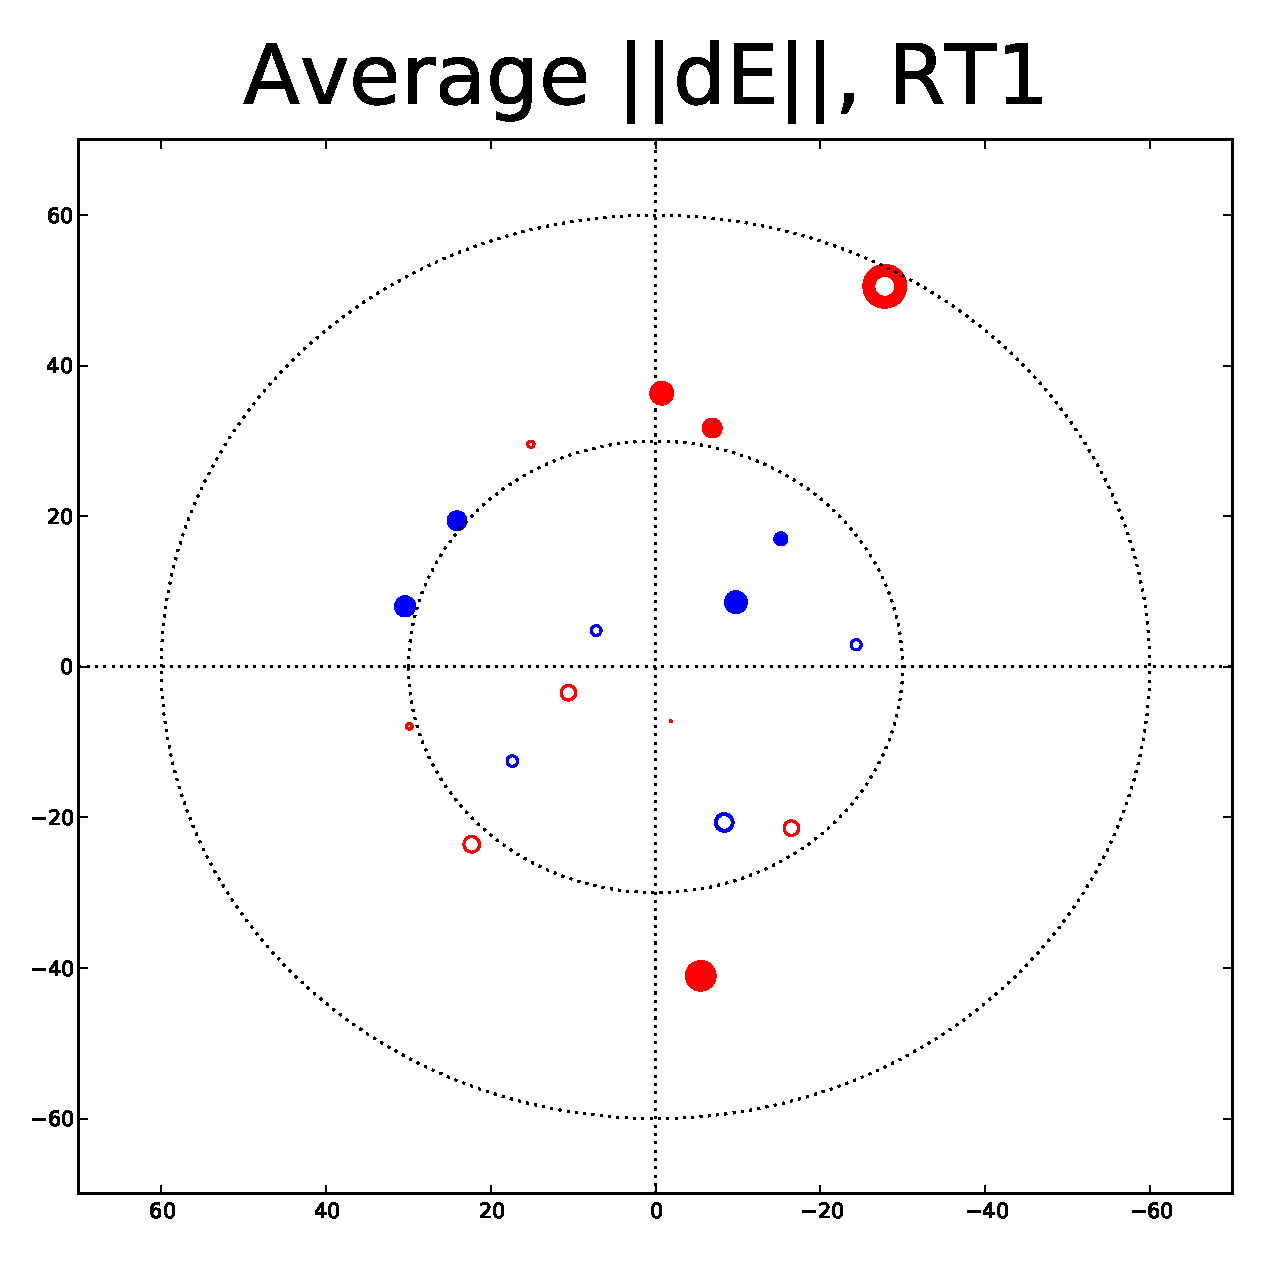
\includegraphics[width=\roguewidth]{qmc2b_dE_ant1} &
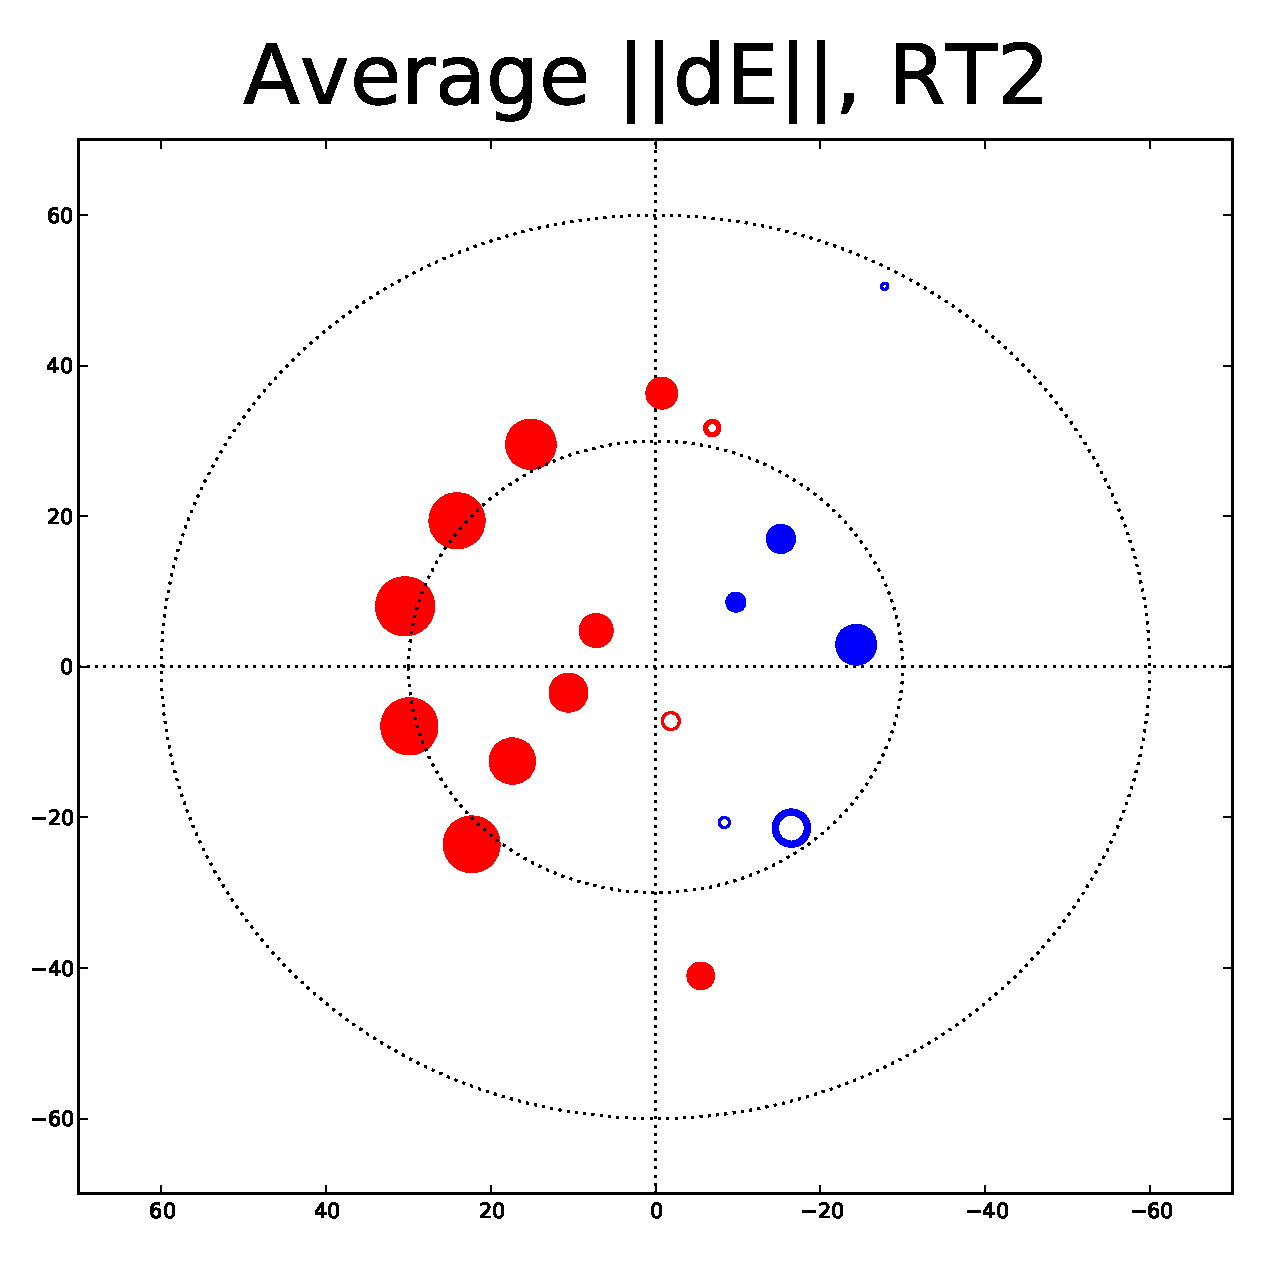
\includegraphics[width=\roguewidth]{qmc2b_dE_ant2} &
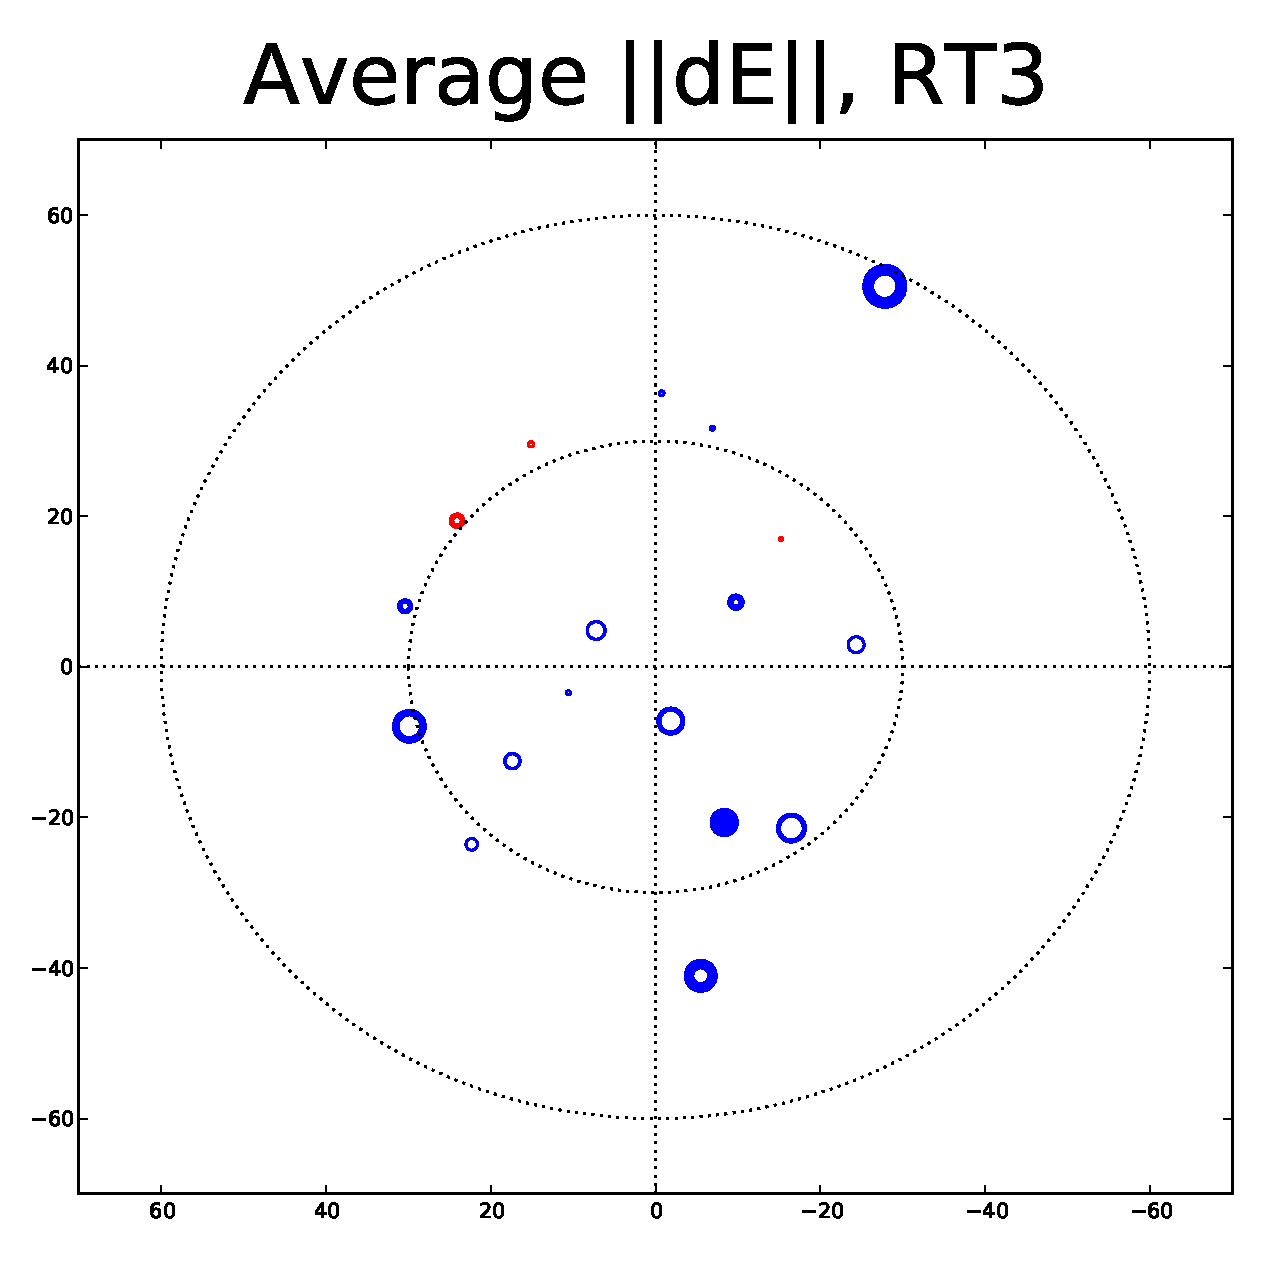
\includegraphics[width=\roguewidth]{qmc2b_dE_ant3} &
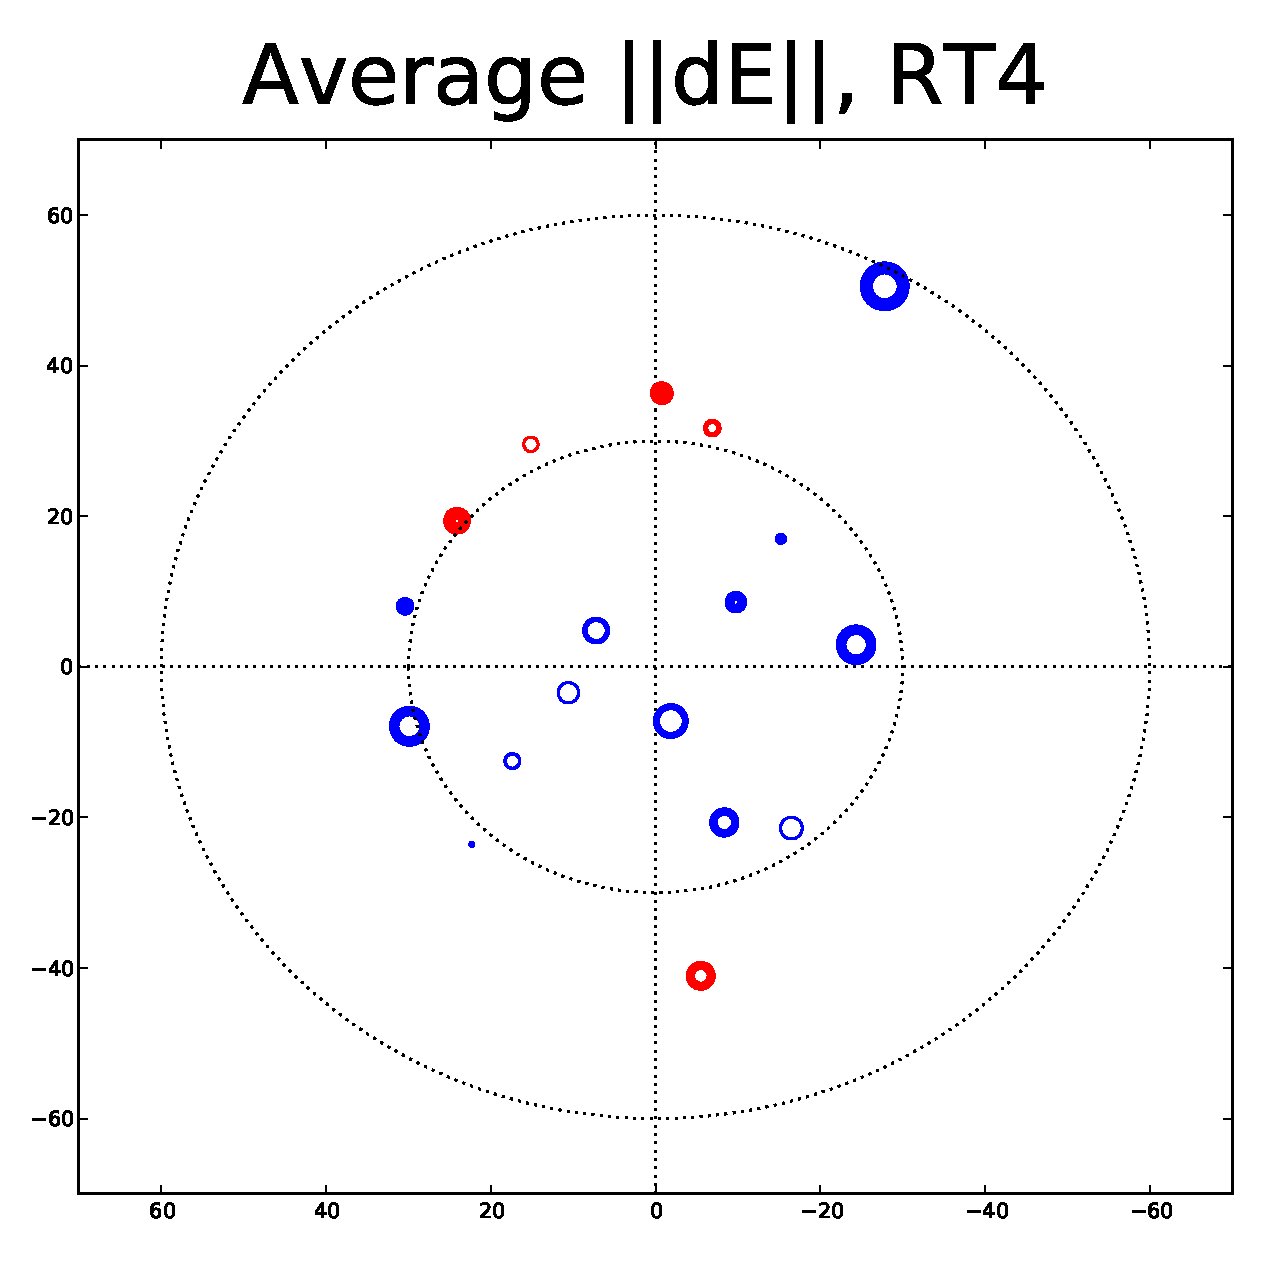
\includegraphics[width=\roguewidth]{qmc2b_dE_ant4} \\
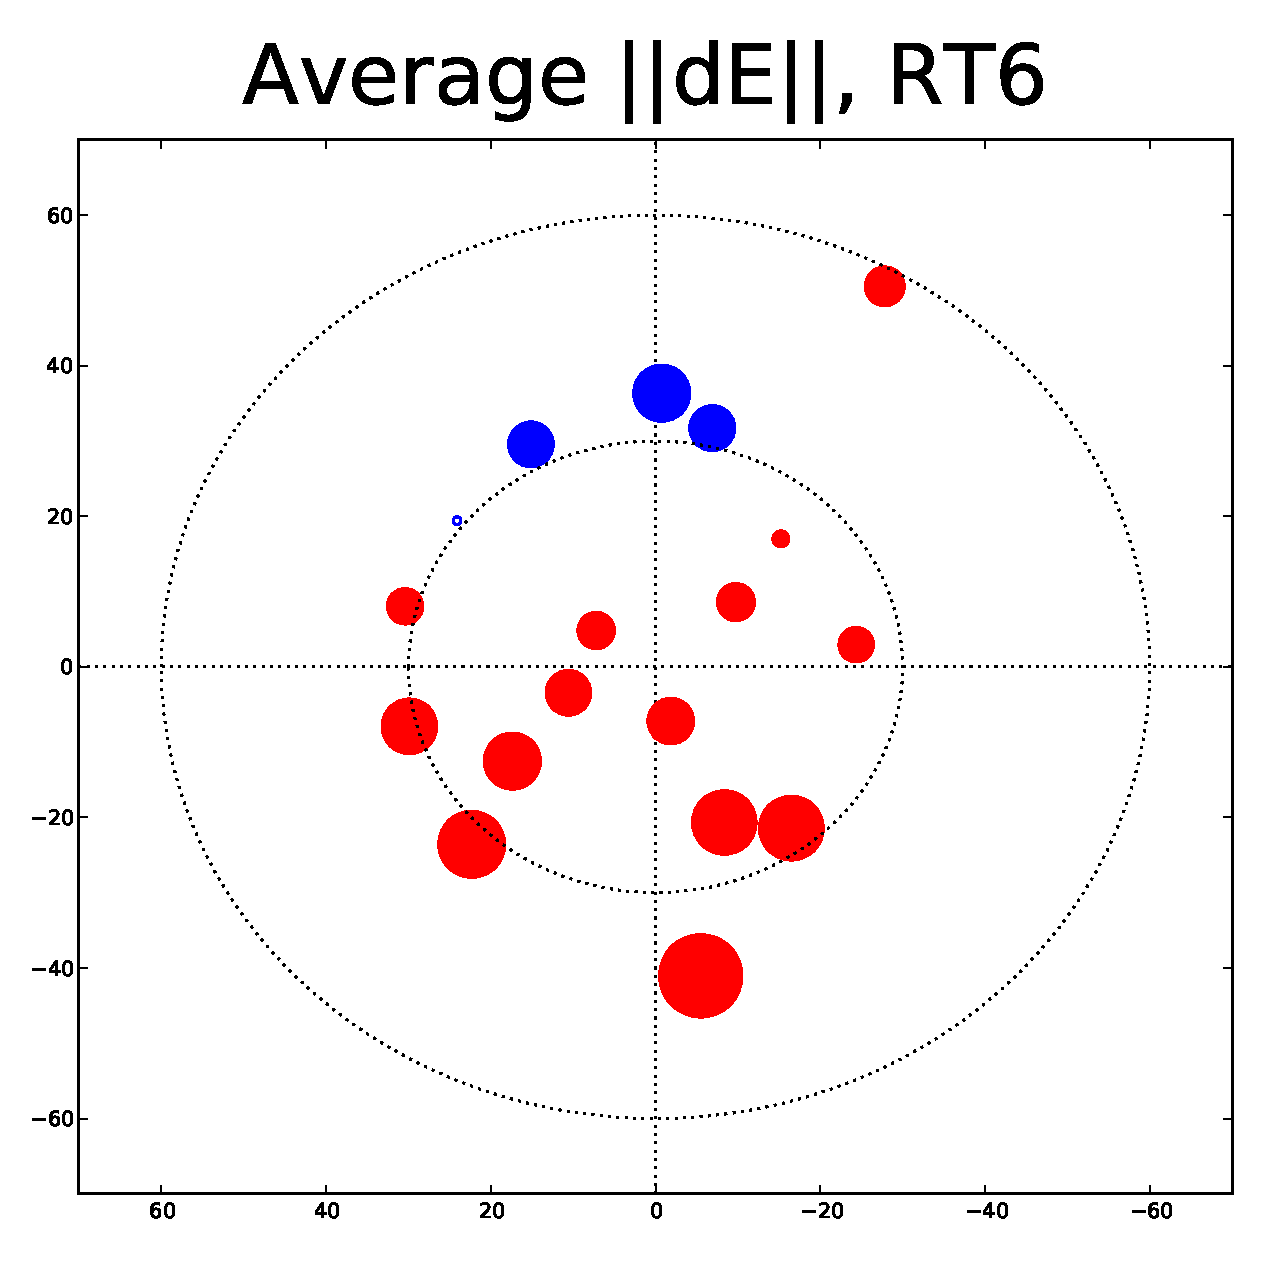
\includegraphics[width=\roguewidth]{qmc2b_dE_ant6} &
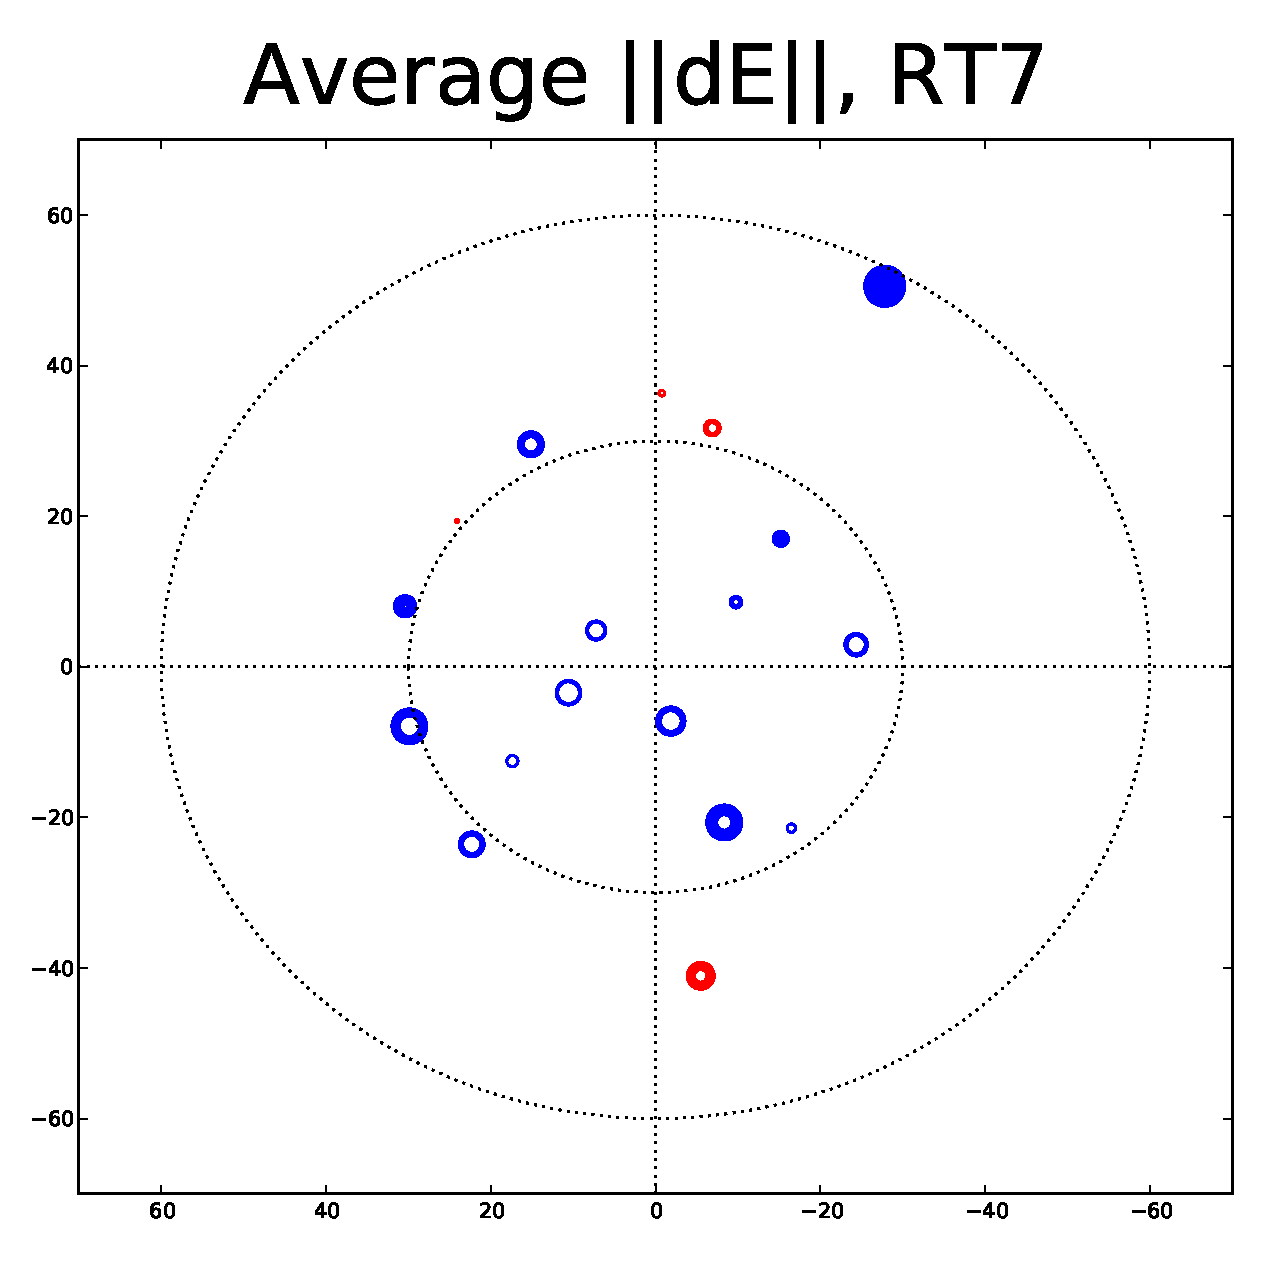
\includegraphics[width=\roguewidth]{qmc2b_dE_ant7} &
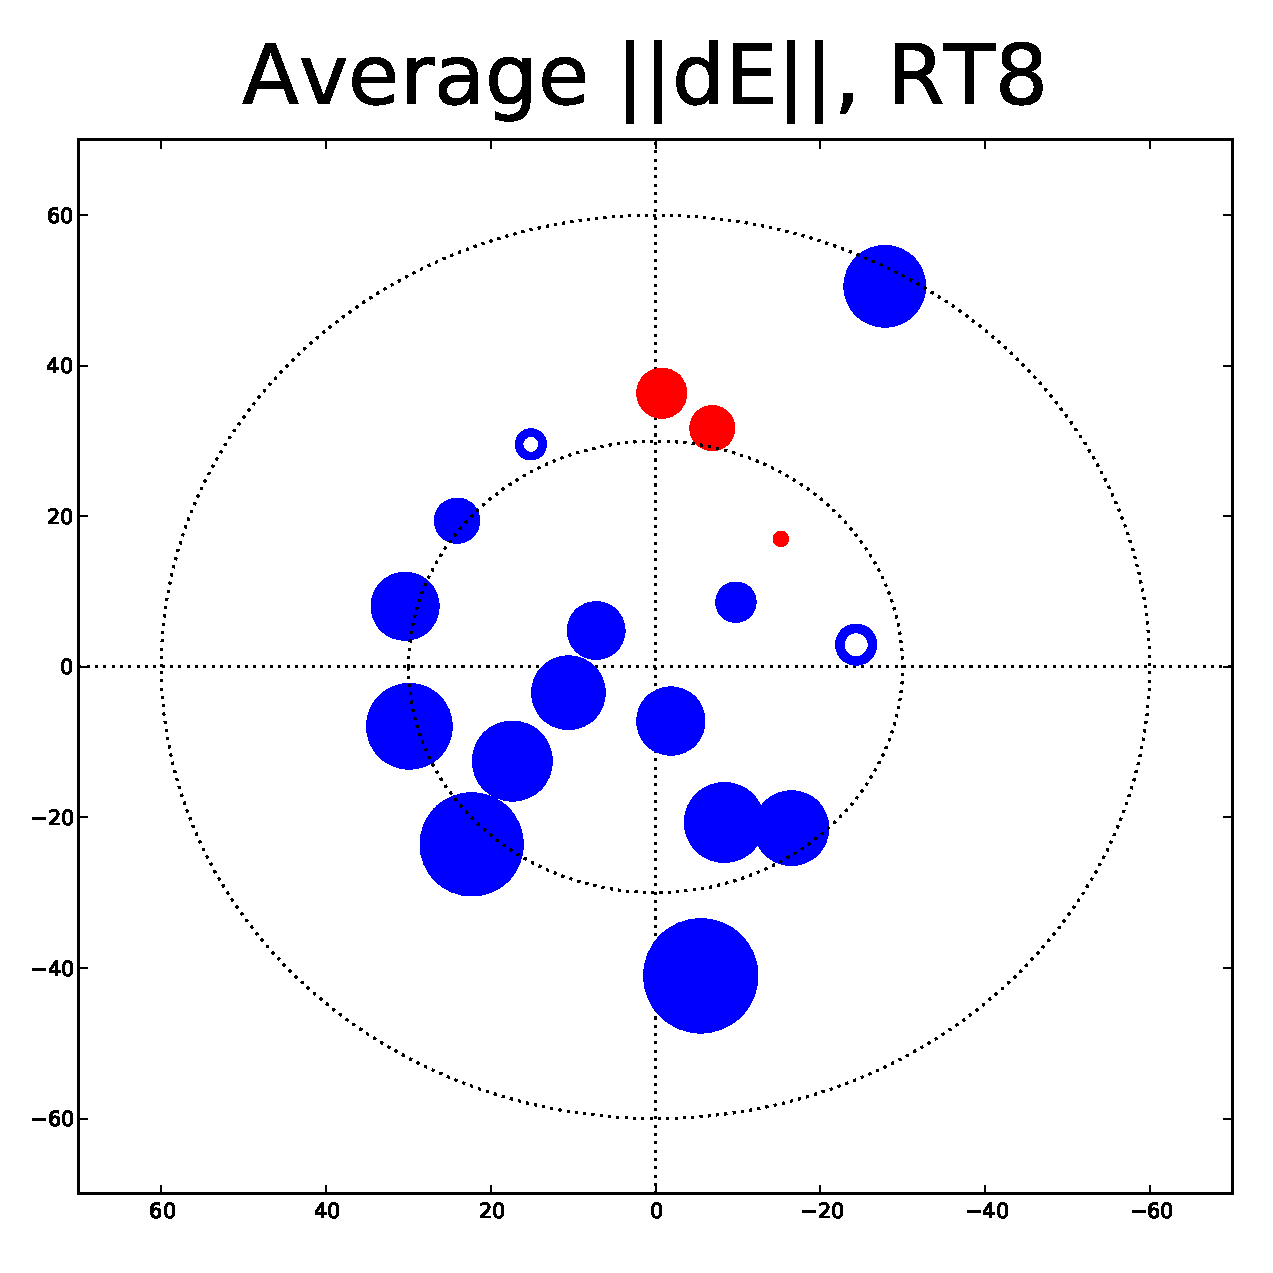
\includegraphics[width=\roguewidth]{qmc2b_dE_ant8} &
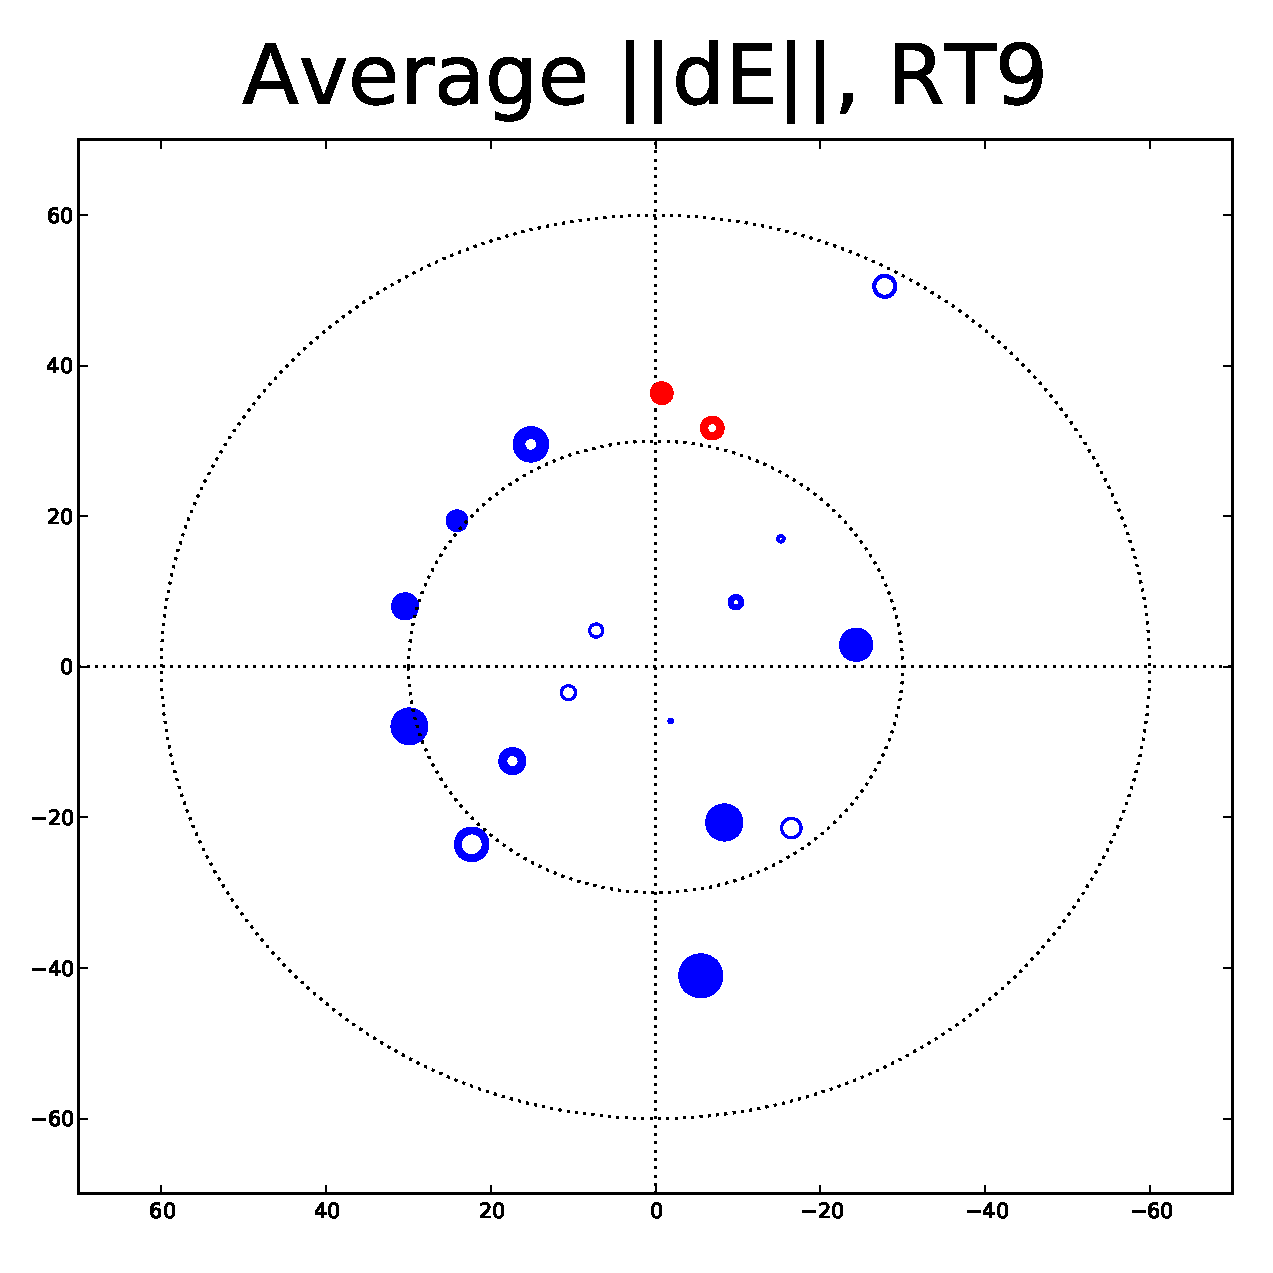
\includegraphics[width=\roguewidth]{qmc2b_dE_ant9} &
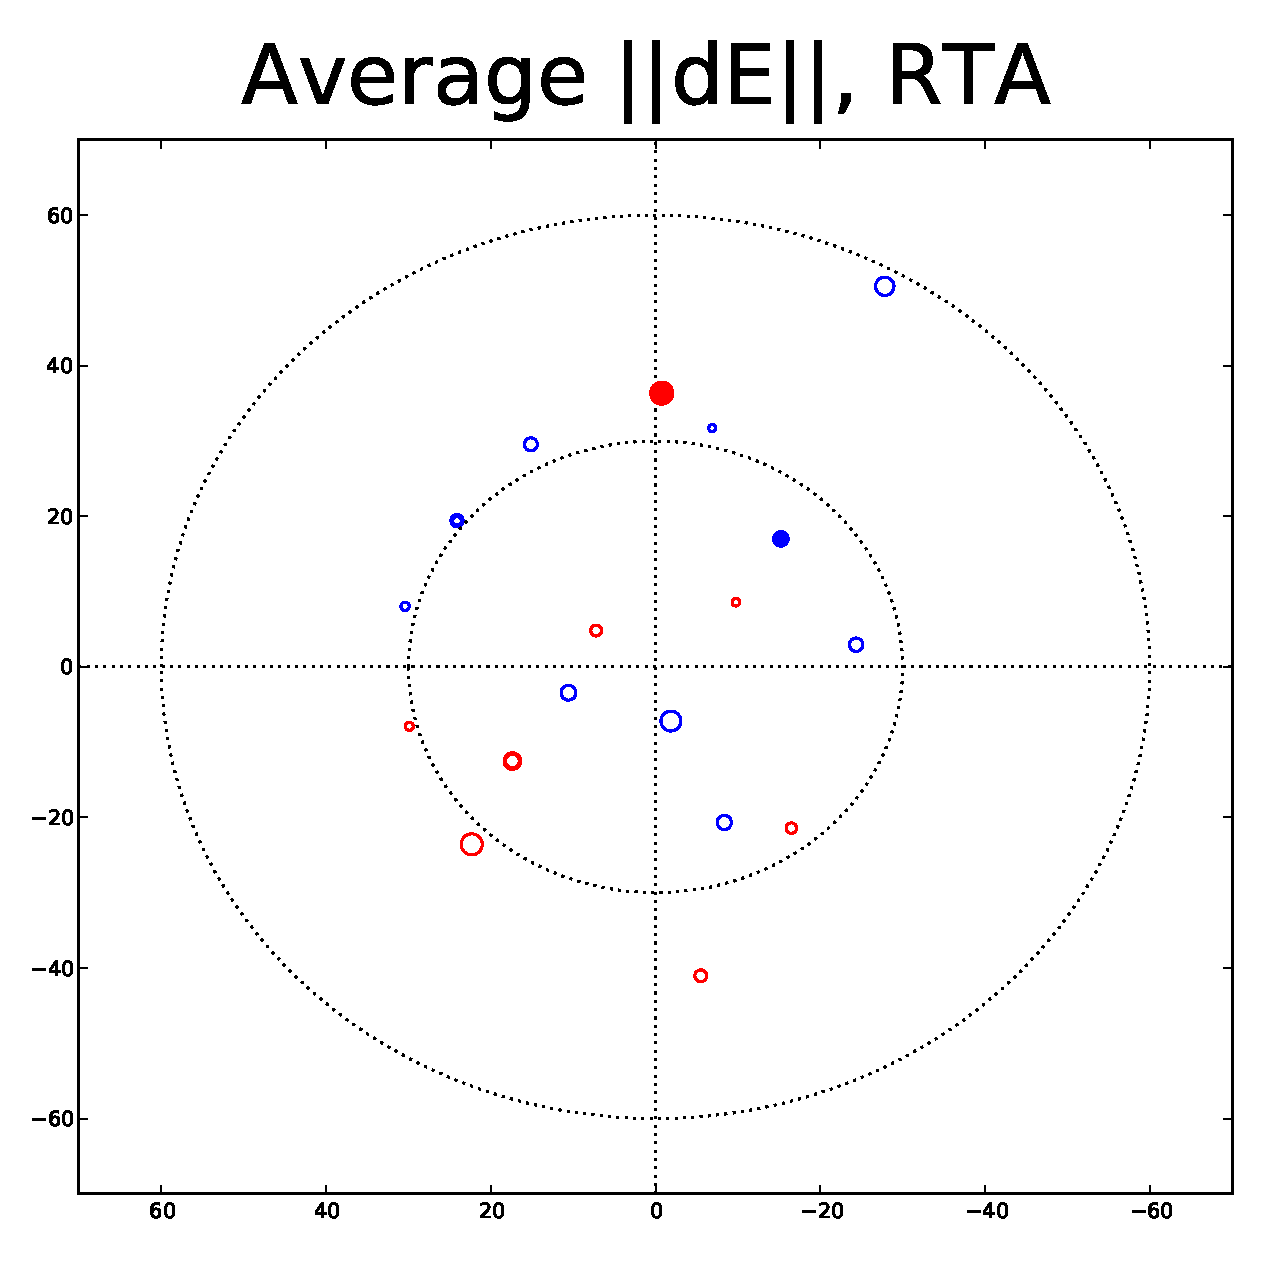
\includegraphics[width=\roguewidth]{qmc2b_dE_antA} \\
&
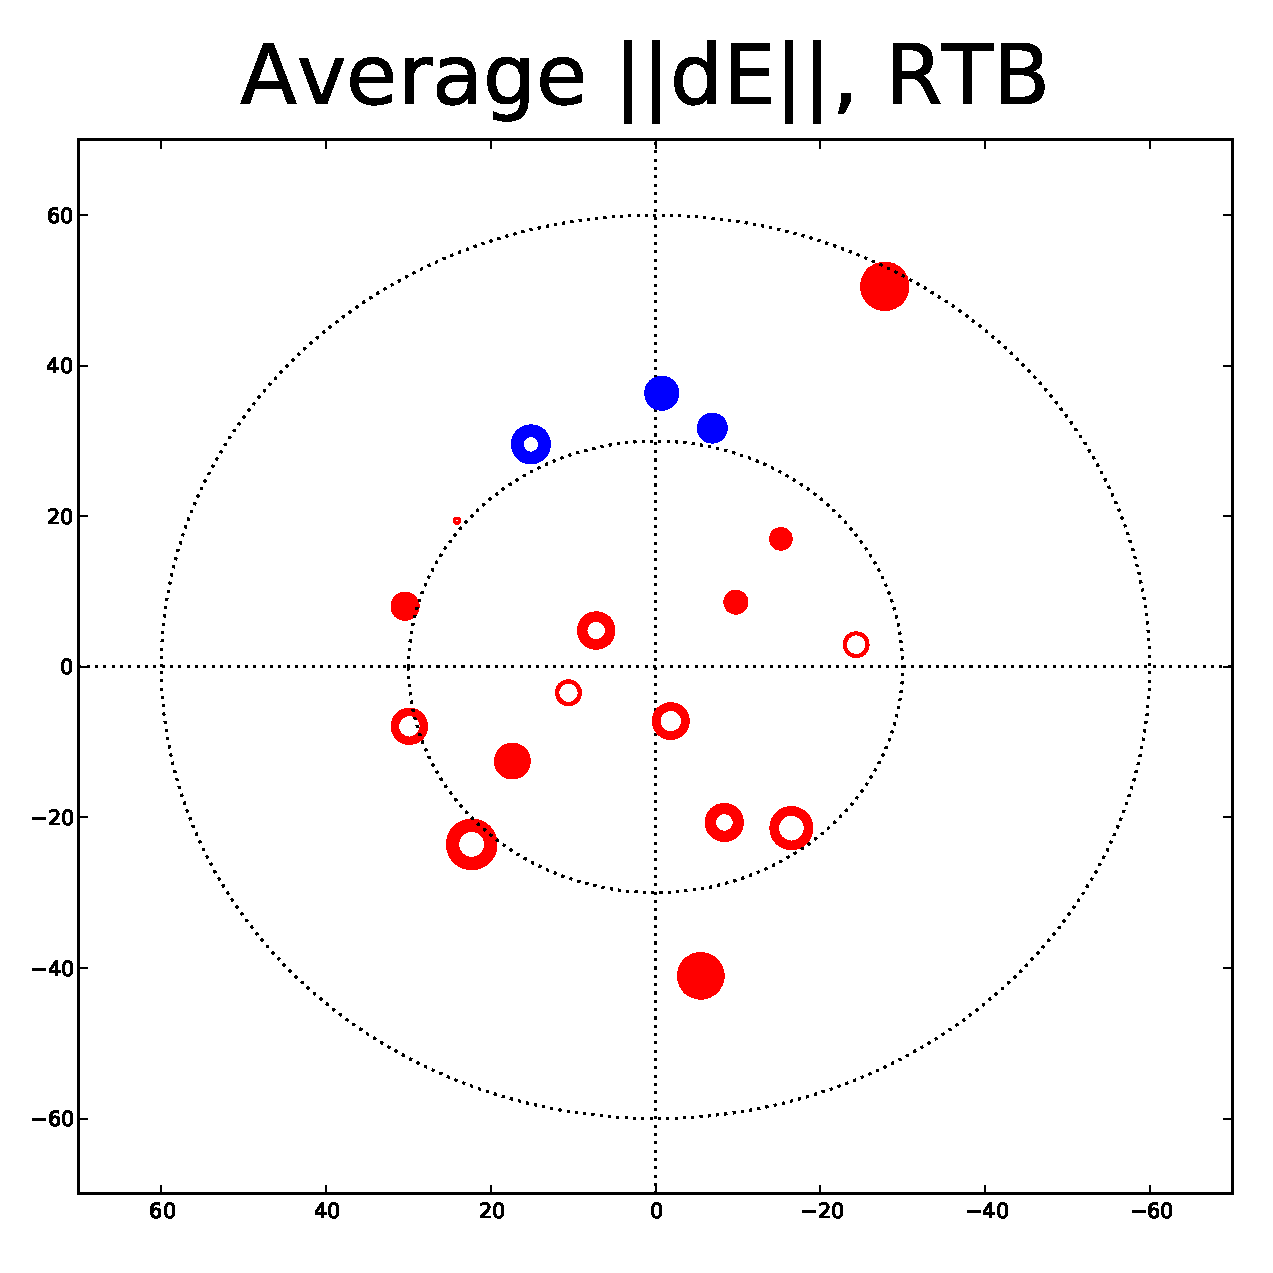
\includegraphics[width=\roguewidth]{qmc2b_dE_antB} &
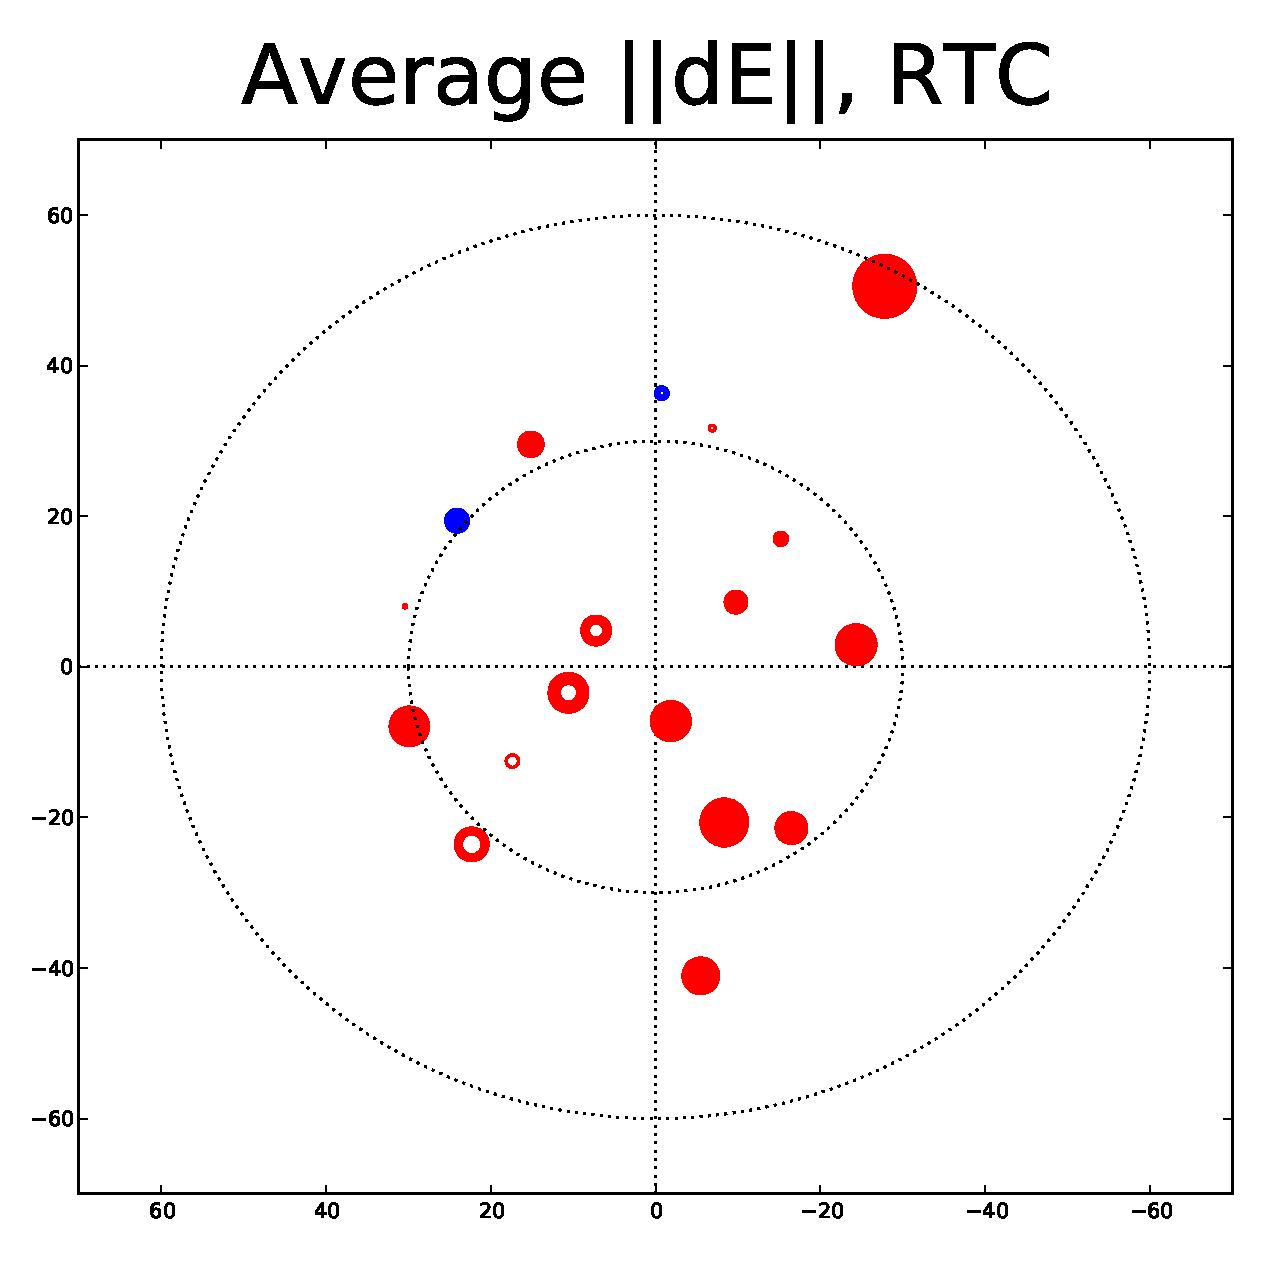
\includegraphics[width=\roguewidth]{qmc2b_dE_antC} &
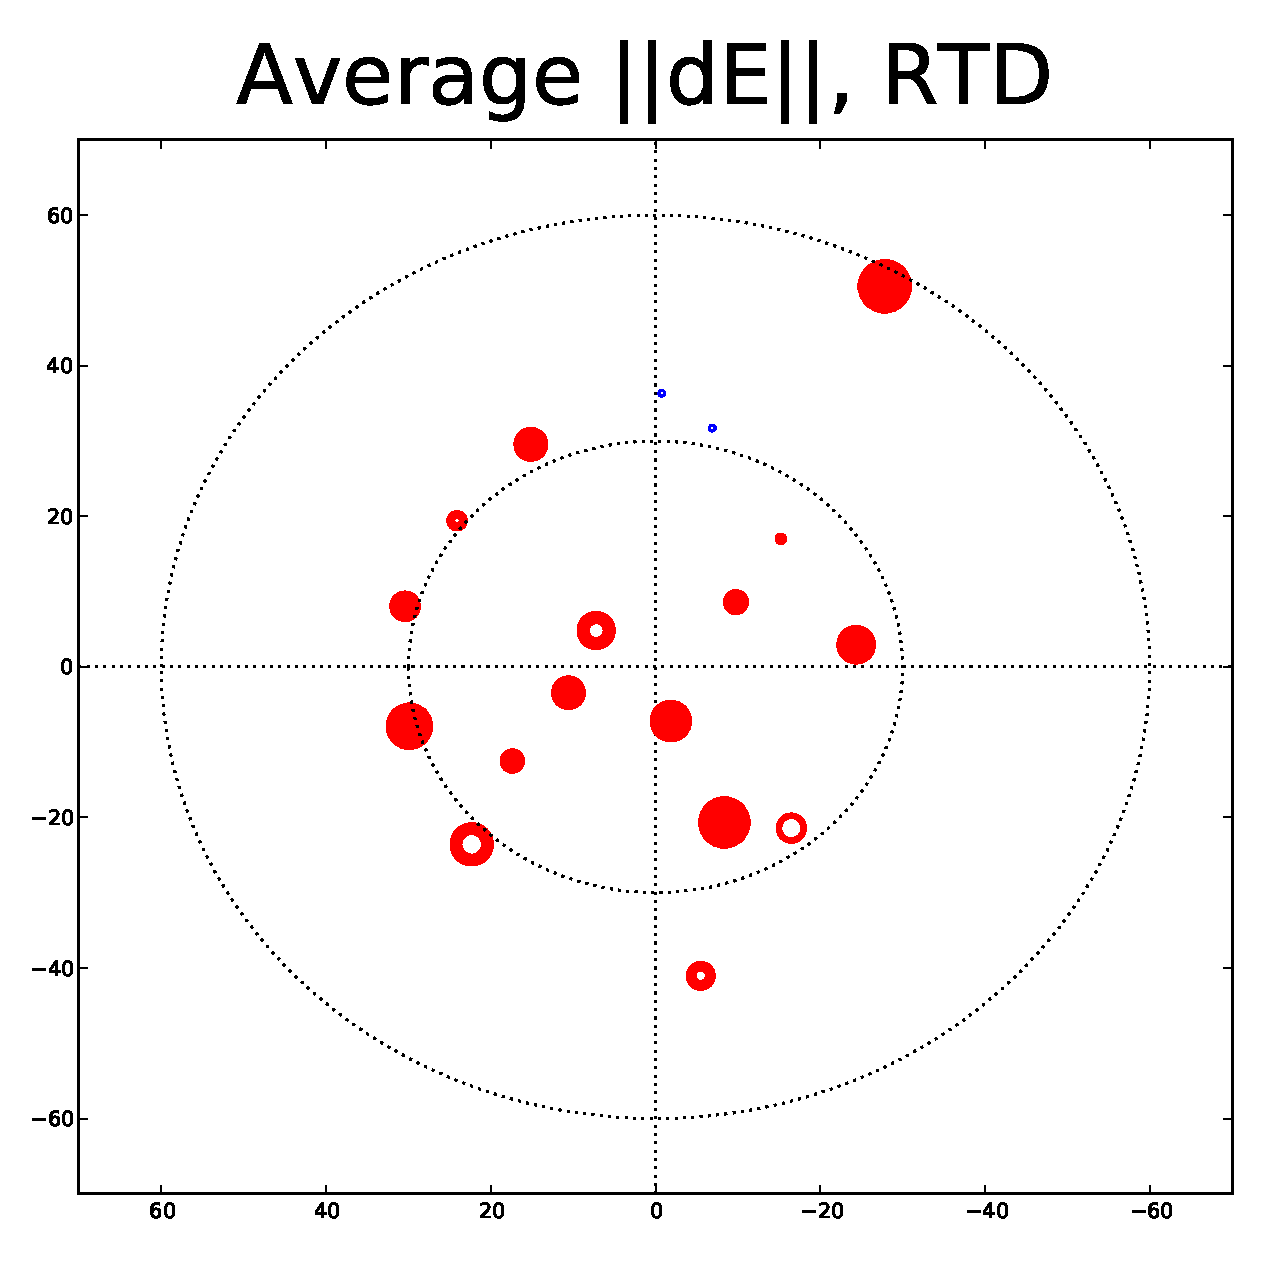
\includegraphics[width=\roguewidth]{qmc2b_dE_antD} 
\end{tabular}
\caption{``Rogues gallery'' plot for the QMC2 Challenge observation. Colours and circle sizes indicate the $\Delta E$ amplitudes towards 18 sources in the QMC2 field, as seen from 13 antennas. Mispointings on RT2, RT6 and RT8 are evident.}
\end{figure}


Once RT8 was fixed, the Challenge observation was carried out. Our $\Delta E$ solutions indicated that four antennas had been mispointed, with one of the mispointings being variable in time. Hans later confirmed that this was exactly right, and that the challenge had been successfully met. Figure 3 shows what we call a ``rogues gallery'' plot of the $\Delta E$-amplitudes. This kind of plot is especially good for detecting mispointings. The circles indicate the average $|\Delta E|$ towards each source, as seen by each antenna. Blue circles correspond to gains above unity (source is brighter than it should be), red circles to gains below unity (source is fainter); the size of the circle shows how far the gain deviates from unity. Static mispointings on RT2, RT6 and RT8 are immediately apparent. The time-variable mispointing on RTB is not as clearly visible in this (time-averaged) plot, but it is obvious on other plots (not shown here.)

Future telescopes, and in particular the SKA, will need to be accurately calibrated for DDEs to achieve their design goals. Such calibration requires a sufficient number of ``beacon'' sources, and it has been a worry whether we have enough suitably bright beacons in the sky. Fortunately, our results suggest that these beacons can be a lot fainter than we thought -- so there's plenty of them everywhere. What may be a luxury problem for the WSRT will be just another day at the office for the SKA!
 

\end{document}